\documentclass{article}
\usepackage[section]{placeins}
\usepackage{graphicx, wrapfig, amsmath, amssymb, physics, hyperref}
\hypersetup{
    colorlinks=true,
    linkcolor=blue,
    filecolor=magenta,      
    urlcolor=cyan,
    }

\author{Yaghoub Shahmari}
\title{Report - Problem Set No 5}
\date{\today}
\graphicspath{ {../Figs/} }

\begin{document}
    \maketitle
    \section*{Problem 1}
    \textbf{Basic description:}

    In this problem, we're going to discuss 2D Random Walkers.
    As the lecture notes described, we expect our results to show these relations:

    \begin{gather*}
        \langle r^{2}\rangle =2dDt,D=\dfrac{l^{2}}{2dr}\\
        R_{g}=\sqrt{\langle r^{2}\rangle },\tau =l=1,d=2\\
        \Rightarrow R_{g}=\sqrt{t}
    \end{gather*}
    
    The simulation creates a list of random choices of steps
    and calculates the sum of total changes of location of the random walker.
    The number of chosen random steps is equal to $t$.
    We repeat the simulation for different $t$ many times
    and calculate the gyration radius of the all of final positions of each $t$.

    \textbf{Results:}

    \begin{figure}[!htb]
        \centering
        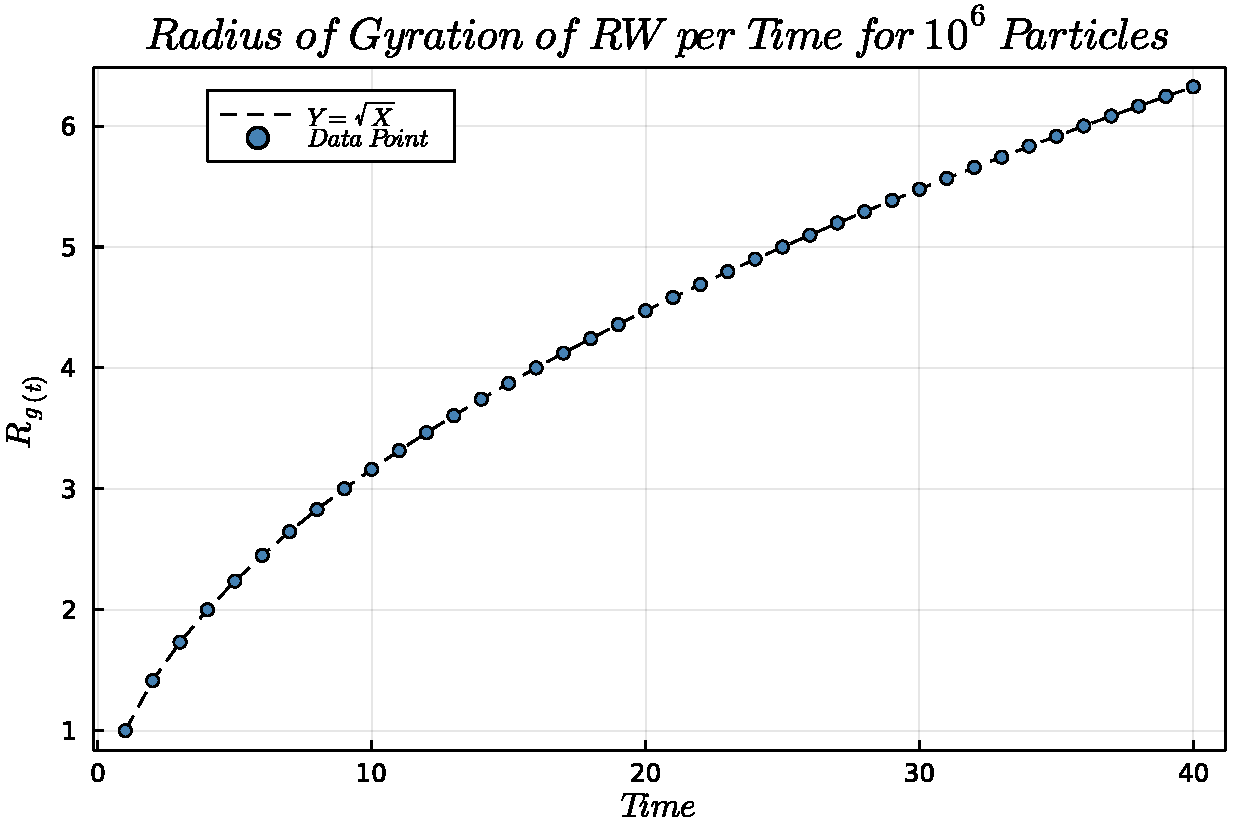
\includegraphics[scale = 0.4]{/Q1/Q1-Rg(t)}
        \label{fig:1.1}
        \caption{Gyration radius of each time step.}
    \end{figure}

    \begin{figure}[!htb]
        \centering
        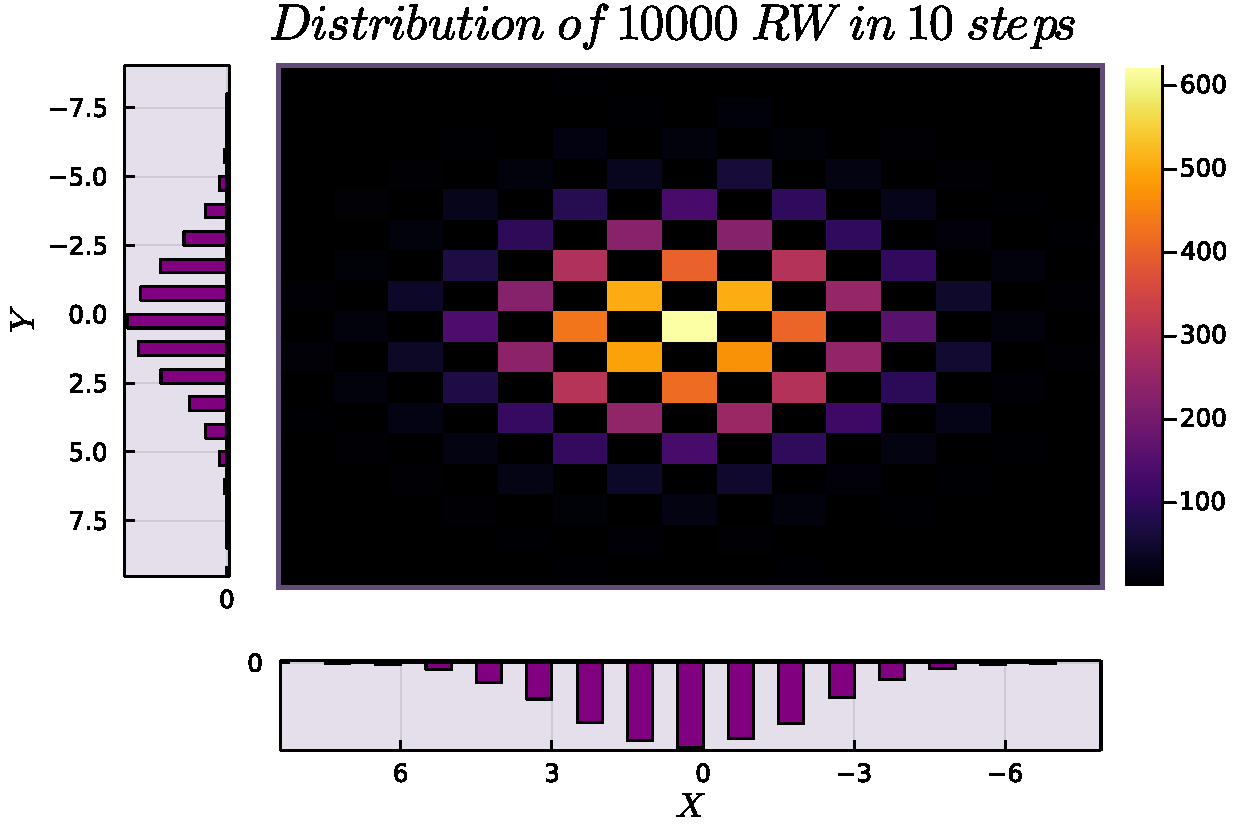
\includegraphics[scale = 0.4]{/Q1/Q1-2DHist1}
        \label{fig:1.2}
        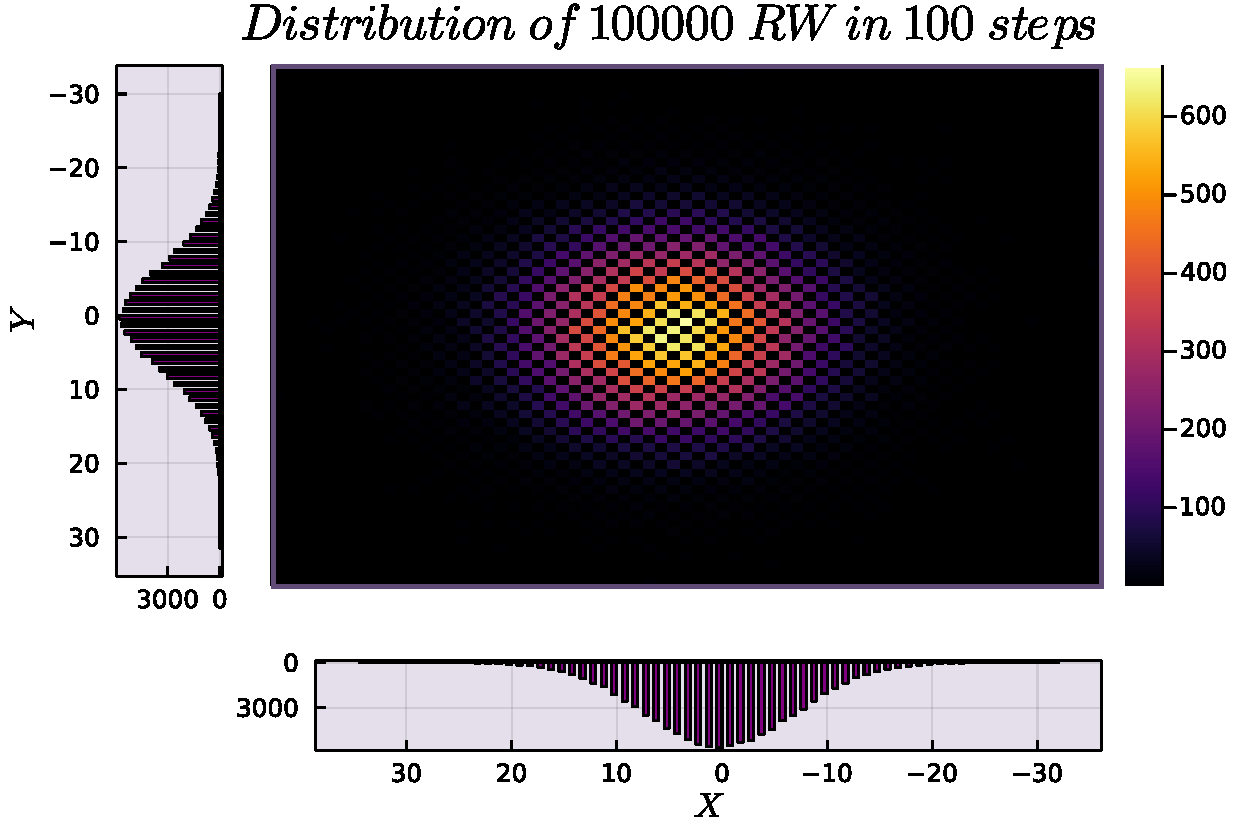
\includegraphics[scale = 0.4]{/Q1/Q1-2DHist2}
        \label{fig:1.3}
        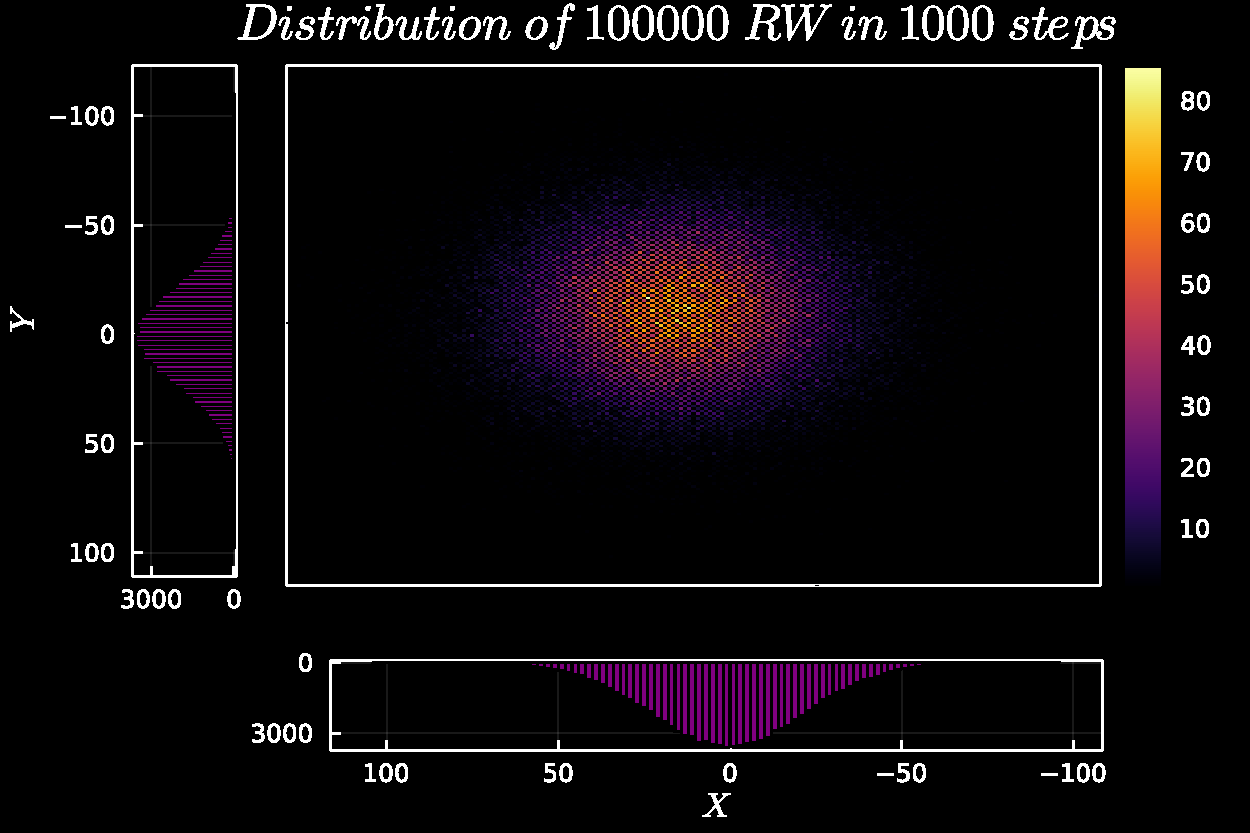
\includegraphics[scale = 0.4]{/Q1/Q1-2DHist3}
        \label{fig:1.4}
        \caption{2D Histogram, Shows distribute of Random Walkers in 10th, 100th, and 1000th time step.}
    \end{figure}

    \pagebreak

    \section*{Problem 2}
    \textbf{Basic description:}

    In this problem, we're going to simulate Diffusion-Limited Aggregation and apply some limitations on 2D Random Walkers.
    We consider a network that has a periodic boundary from sides,
    a fixed floor, and a non-fixed boundary on top.
    We continue to release particles until the roof reaches a specific location.
    
    \textbf{Results:}

    \begin{figure}[!htb]
        \centering
        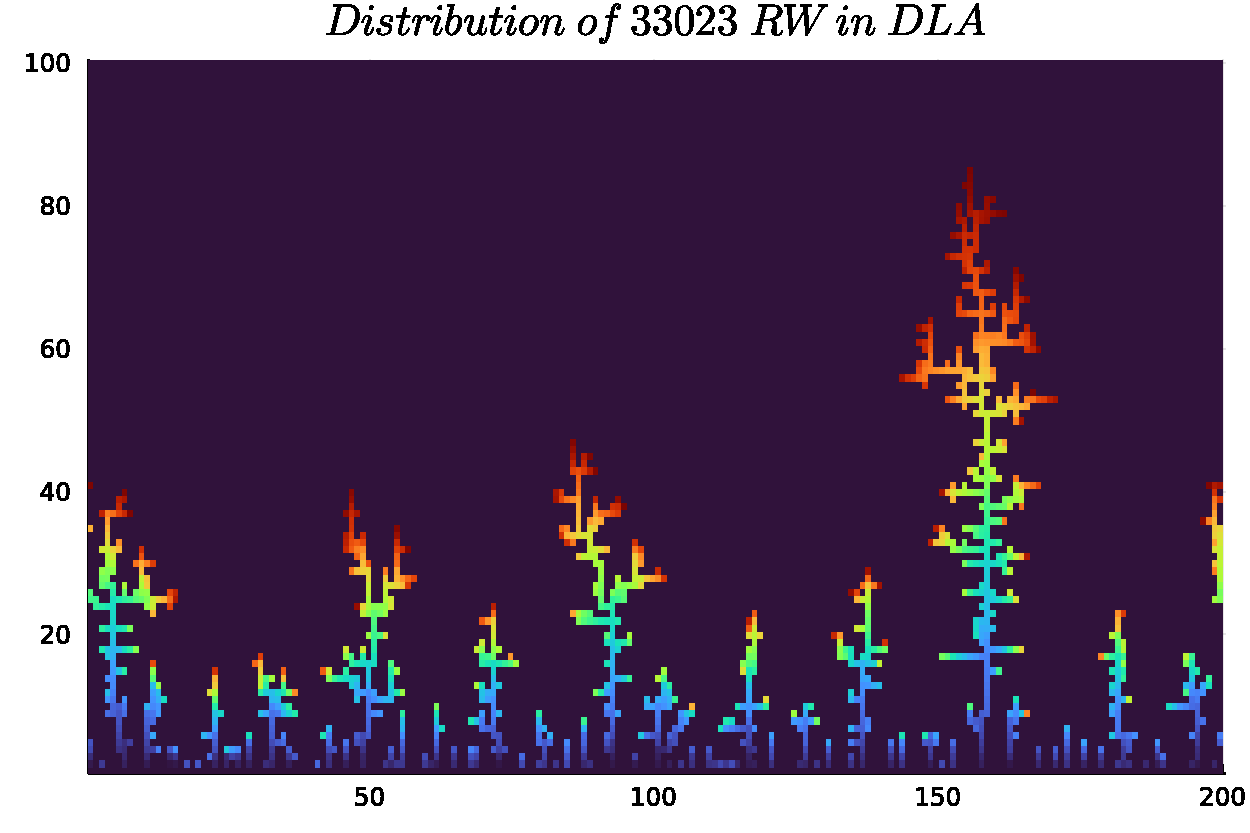
\includegraphics[scale = 0.4]{/Q2/Q2-HM}
        \label{fig:2.1}
        \caption{Distribution of Diffusion-Limited Aggregation. An animation is provided in Figs folder.}
    \end{figure}

    \pagebreak

    \section*{Problem 3}
    \textbf{Basic description:}

    In this problem,
    we're going to count the number of Self-Avoiding Walks of a Random walker.
    A normal random walker has a $4^N$ possible way to navigate $N$ step on a surface.
    It is a simple permutation of 4 choices.
    To find every possible way of navigation using an algorithm,
    we need N fors to check every way.
    Instead of using N fors we can just call a rescue function
    that calls itself within itself exactly N times.
    If we check avoidance then call the function,
    we can count the number of Self-Avoiding Walks.
    
    \textbf{Results:}

    \begin{figure}[!htb]
        \centering
        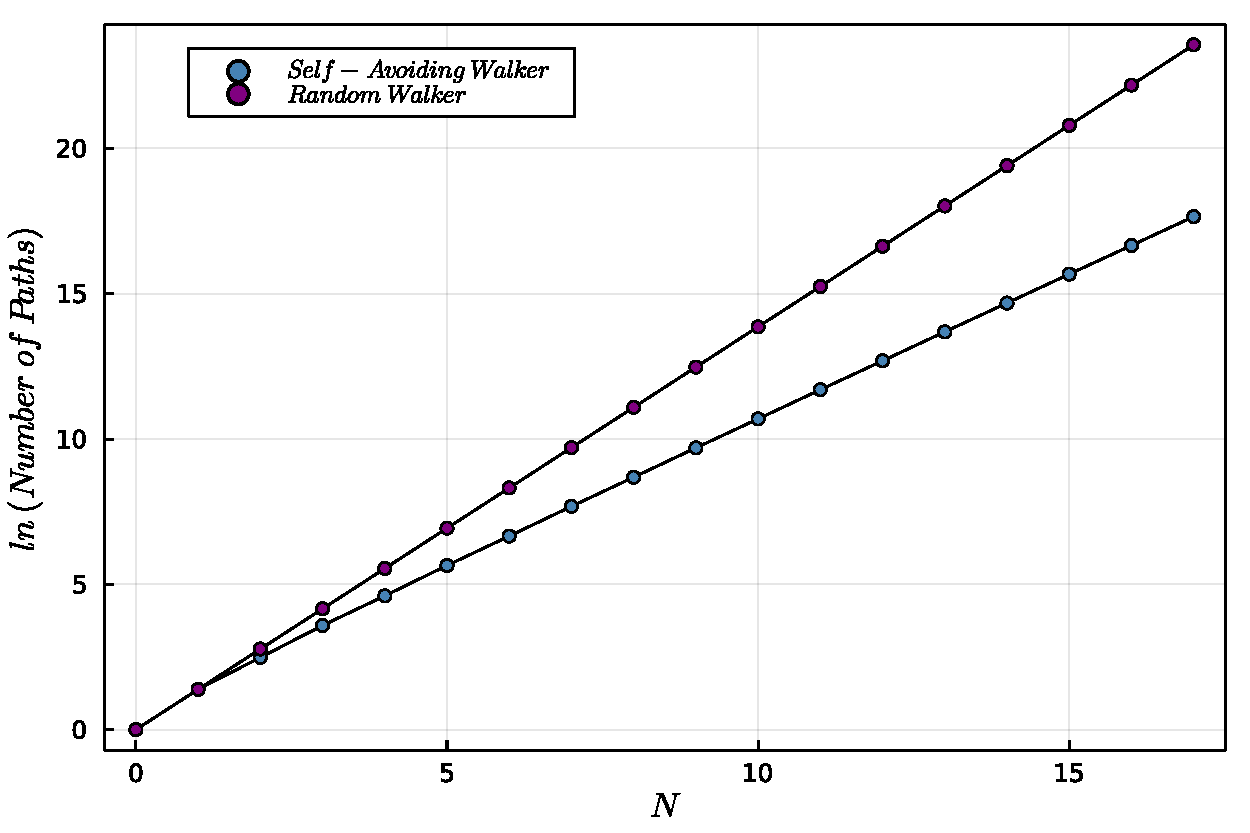
\includegraphics[scale = 0.25]{/Q3/Q3-1}
        \label{fig:3.1}
        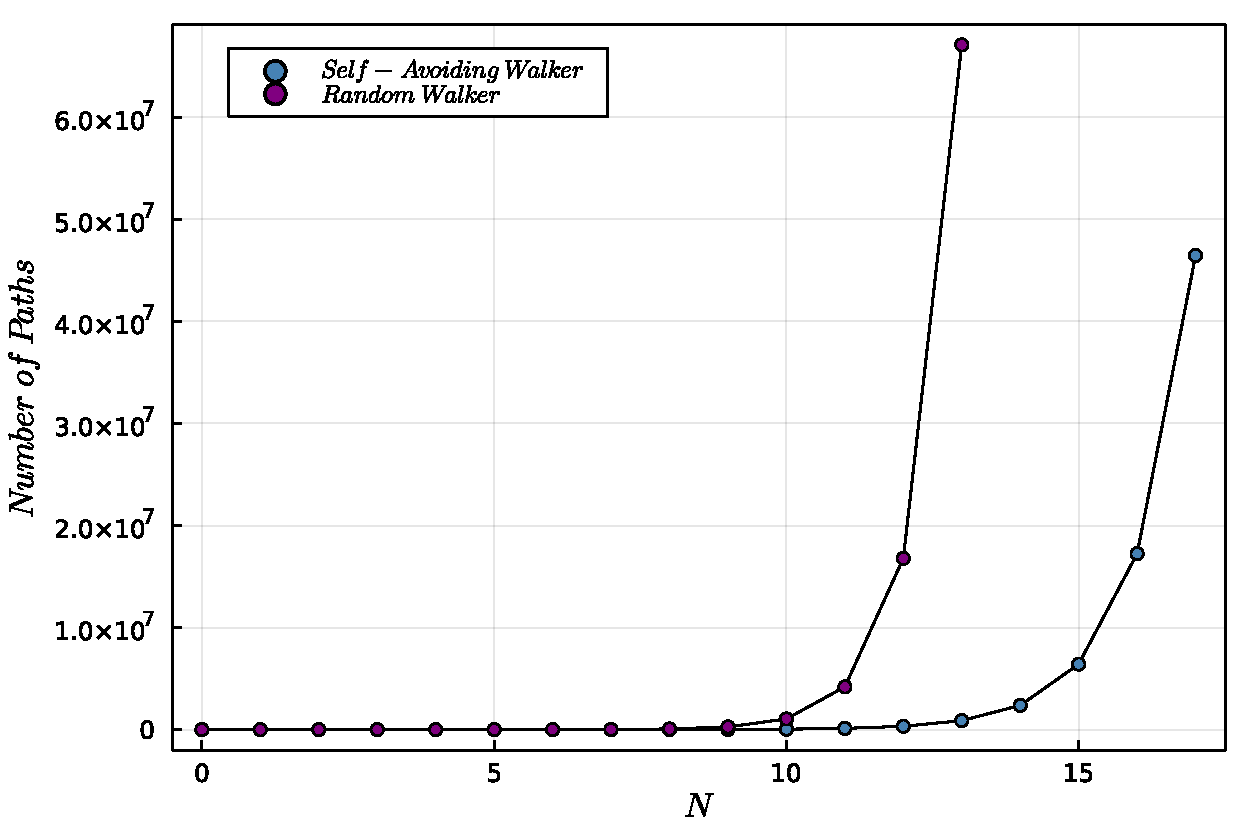
\includegraphics[scale = 0.25]{/Q3/Q3-2}
        \label{fig:3.2}
        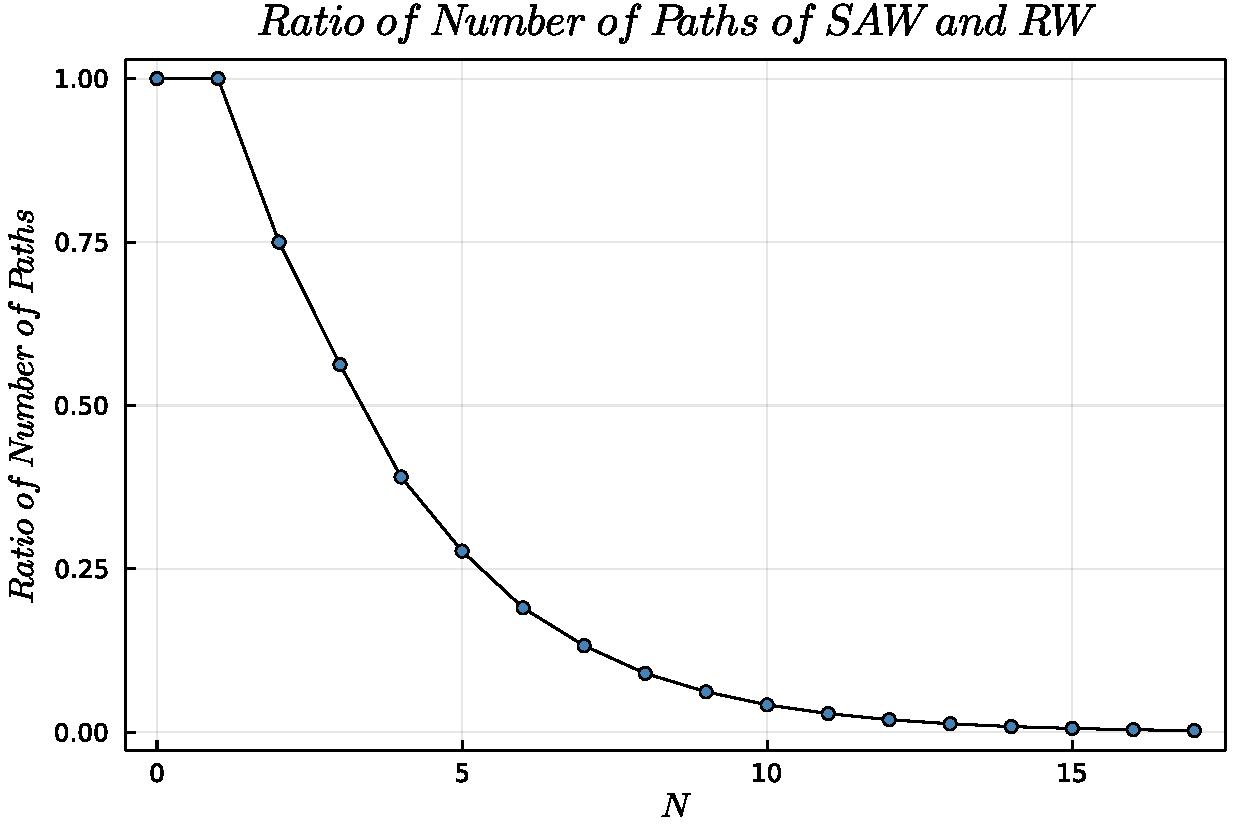
\includegraphics[scale = 0.5]{/Q3/Q3-3}
        \label{fig:3.3}
        \caption{Plots (log-log and normal scale plot and ratio plot) that shows the growth of the count of ways.}
    \end{figure}

    \pagebreak

    \section*{Problem 4}
    \textbf{Basic description:}

    In this problem, we're going to study the Random number generator.
    Initially, we make a sample of random numbers in [0,9] and show the distribution.
    Then check the coefficient of variation and its relation to the value of N.
    
    \textbf{Results:}

    \begin{figure}[!htb]
        \centering
        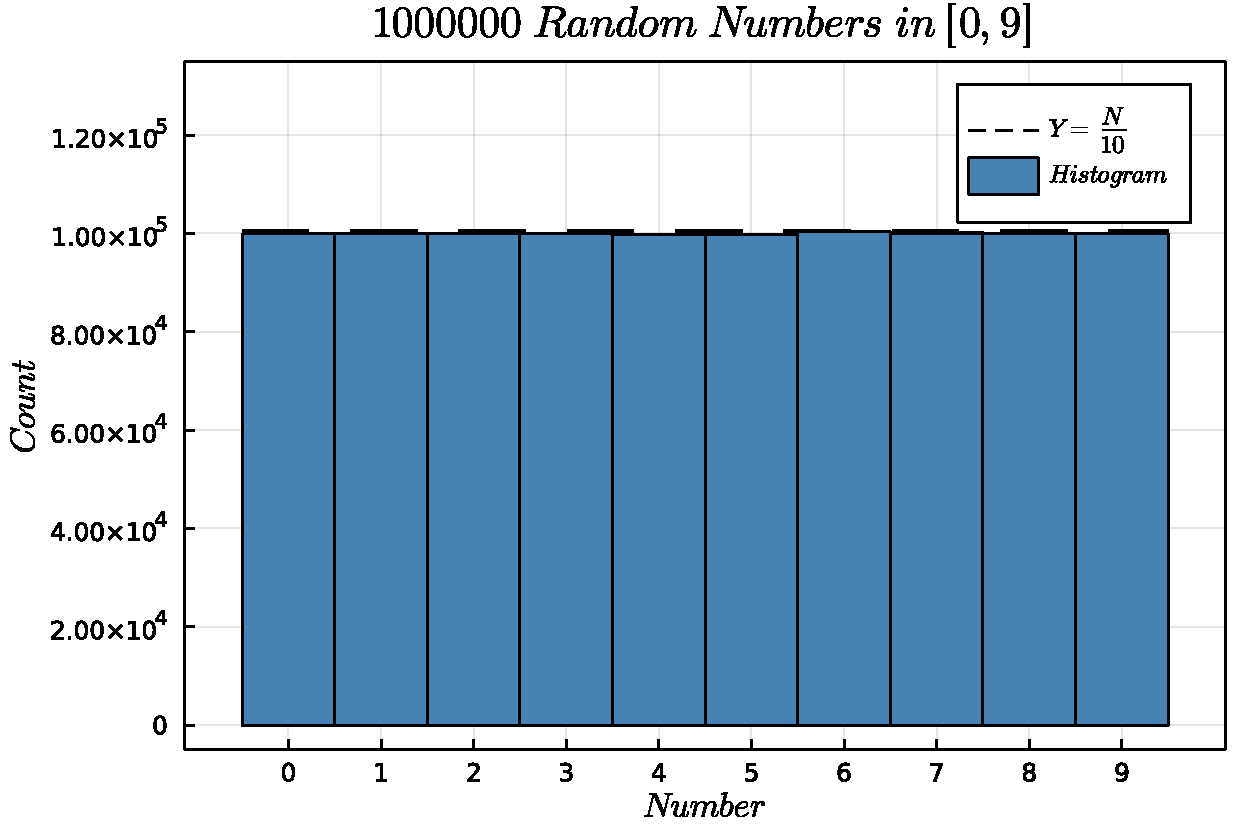
\includegraphics[scale = 0.4]{/Q4/Q4-Hist}
        \label{fig:4.1}
        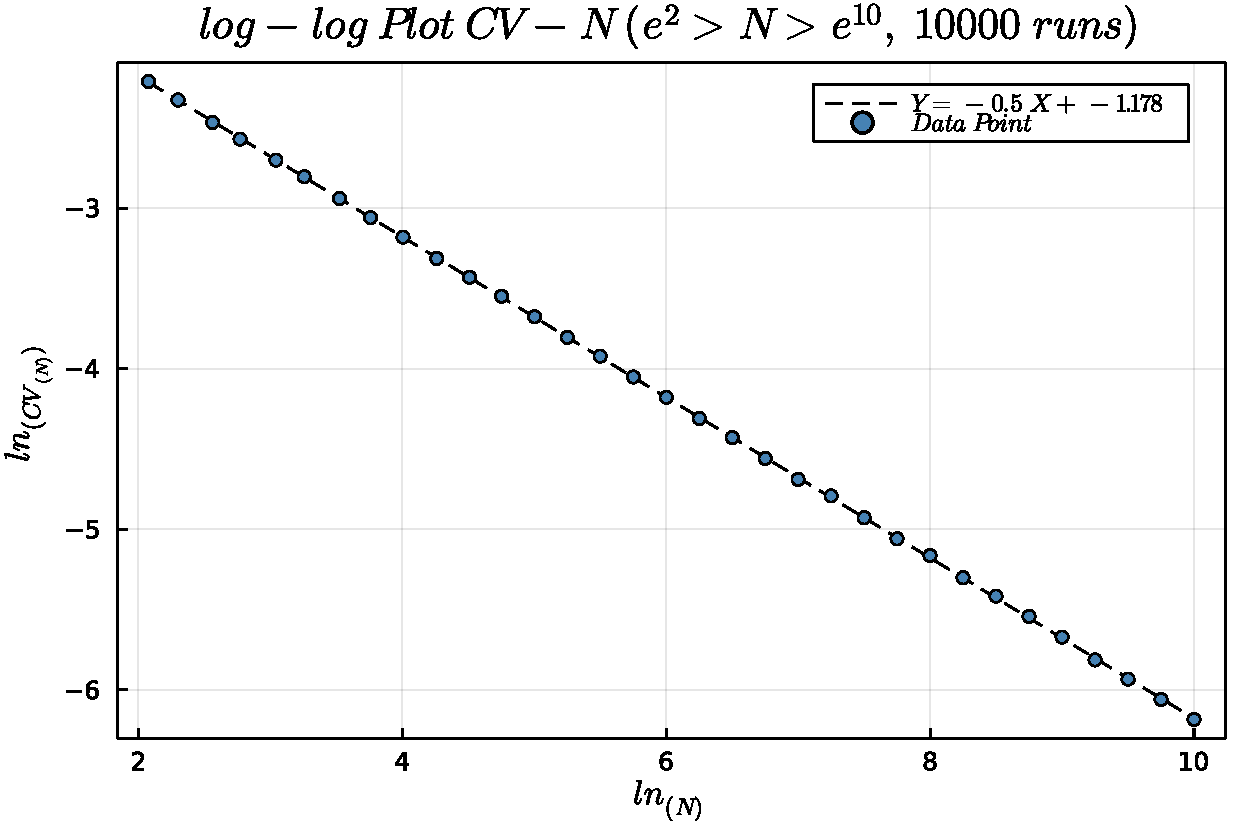
\includegraphics[scale = 0.4]{/Q4/Q4-Scat}
        \label{fig:4.2}
        \caption{As you can see, the data shows the distribution of Numbers follows the $Y = \frac{N}{10}$ and for CV we have $\frac{\sigma}{N}~N^{-0.5}$}
    \end{figure}

    \pagebreak

    \section*{Problem 5}
    \textbf{Basic description:}

    In this problem, we do the same thing we have done for the previous Question,
    but instead of analyzing the sample we gathered from the random generator,
    we sample the numbers. We only choose the numbers came before the 4.

    \textbf{Results:}

    \begin{figure}[!htb]
        \centering
        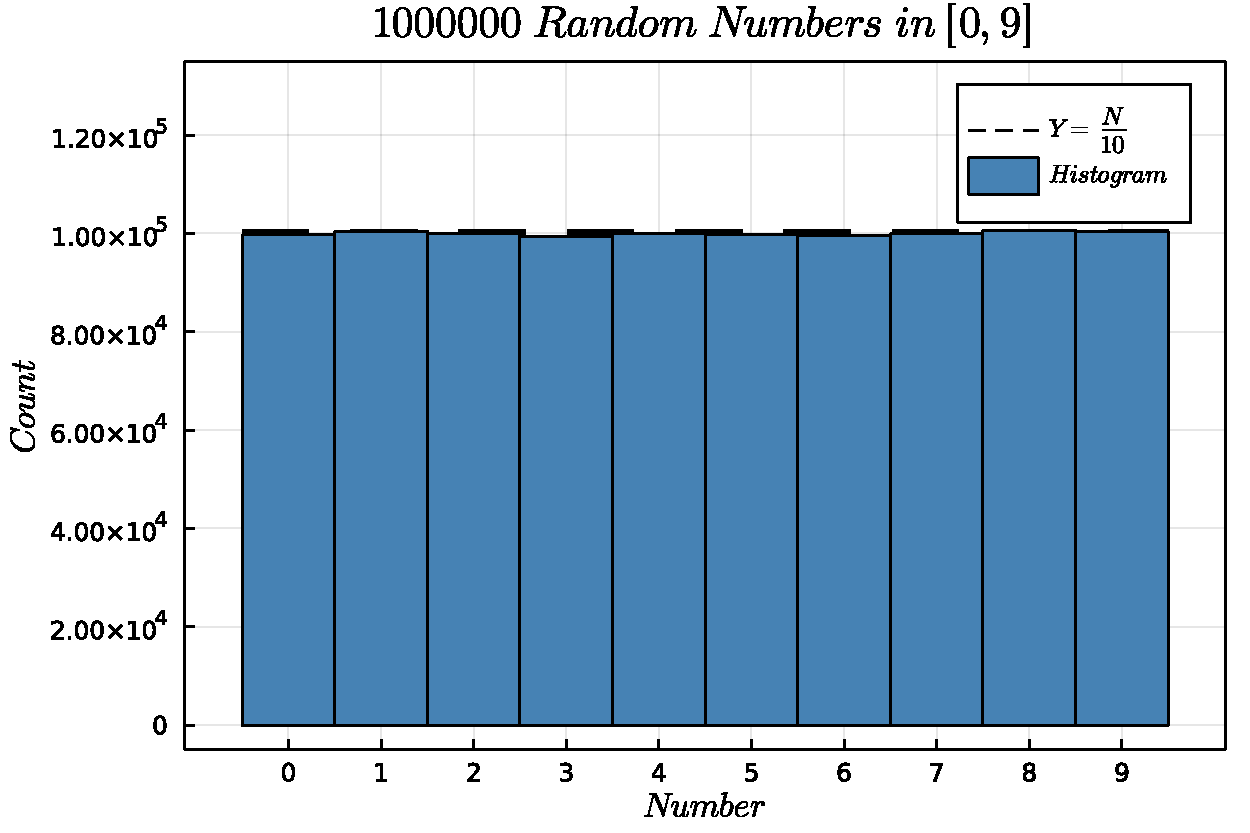
\includegraphics[scale = 0.4]{/Q5/Q5-Hist}
        \label{fig:5.1}
        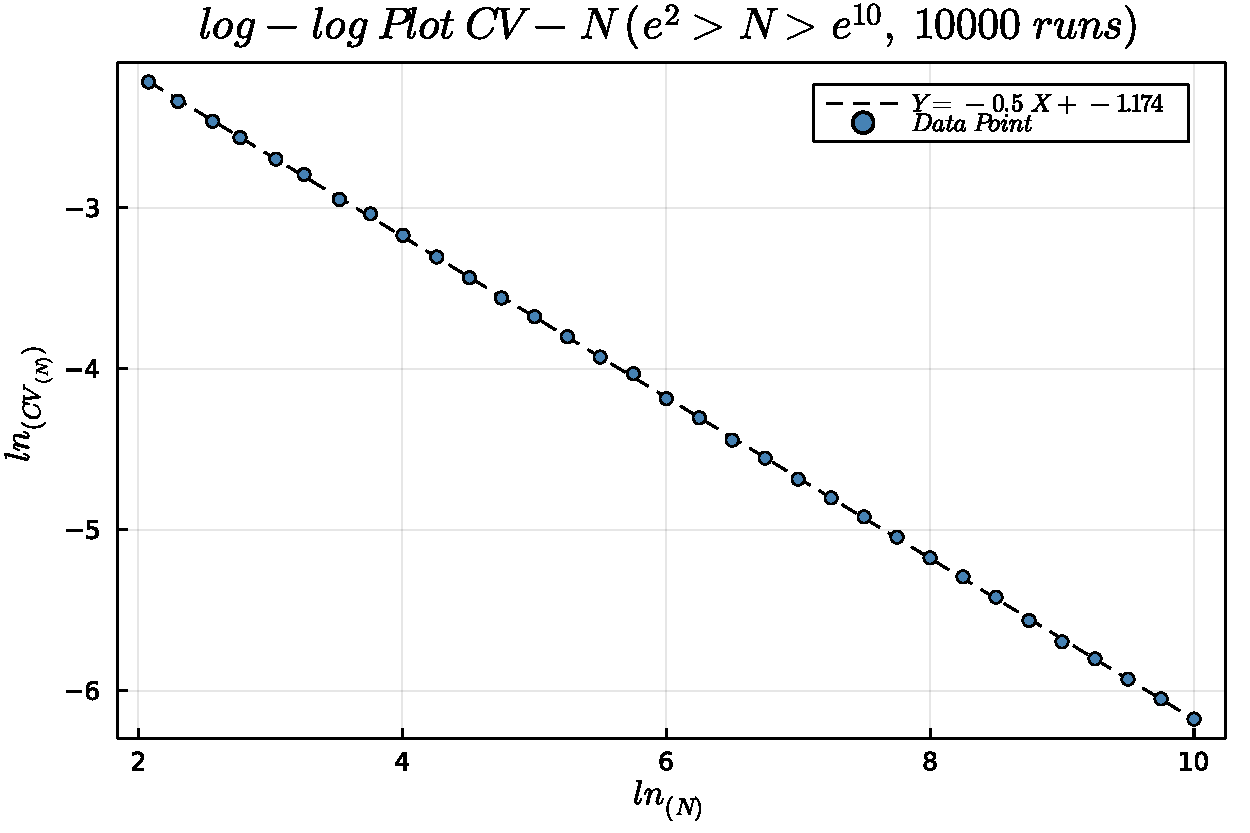
\includegraphics[scale = 0.4]{/Q5/Q5-Scat}
        \label{fig:5.2}
        \caption{As you can see, the data shows the distribution of Numbers follows the $Y = \frac{N}{10}$ and for CV we have $\frac{\sigma}{N}~N^{-0.5}$}
    \end{figure}

    \pagebreak

    \centering
    \textbf{The whole data I gathered is in \href{https://github.com/shahmari/ComputationalPhysics-Fall2021/tree/main/ProblemSet5/Data}{this link}}
    
    \textbf{Also check \href{https://www.youtube.com/watch?v=dQw4w9WgXcQ}{this link}}

    Thanks for watching :)
\end{document}